% =============================================================================
% File:  intro_git.tex -- Introduction to Git 
%
% =============================================================================

\documentclass[10pt,xcolor=dvipsnames]{beamer}

\usetheme{Madrid}

%\renewcommand\mathfamilydefault{\rmdefault}
\usefonttheme[onlymath]{serif}

%\usecolortheme{seahorse}
\usepackage[utf8]{inputenc}
\usepackage{xcolor}
\usepackage{colortbl}
\usepackage{verbatim}
\usepackage{hyperref}
%gets rid of bottom navigation bars
\setbeamertemplate{footline}{}
%gets rid of navigation symbols
\setbeamertemplate{navigation symbols}{}
%\usetheme{Frankfurt}
%\usetheme{Rochester}
%\usepackage{beamerthemeshadow}

% \usepackage{amsmath}
% \usepackage{amssymb}

%\usepackage{floatflt}
%\usepackage[utf8]{inputenc}
%\usepackage{multirow}
    \usepackage{mathptmx}
\graphicspath{{./pics/}{./figs/}}
\usepackage{graphicx}          % Include this line if your 
                               % document contains figures,
\usepackage[super]{nth}
\usepackage{multirow}
\usepackage{amsmath}
\usepackage{verbatim}


\AtBeginSection[]
{
  \frame{
    \frametitle{Summary}
    {\scriptsize\tableofcontents[currentsection]}
  }
}


%%%%%%%%%% Header %%%%%%%%%%%%
\title{Short Introduction to Git}
\subtitle{Grup Seminar}

\author{Andr\'as Hartmann, Sascha Zickenrott}
\institute[LCSB]{
LCSB, Computational Biology group
  University of Luxembourg
}
% Mandatory to **declare** a logo to be placed on the bottom right -- normally the
% university logo. ADAPT ACCORDINGLY:

\date[June 29, 2016]{June 29, 2016, Luxembourg}

\logo{
\includegraphics[height=0.10\paperheight]{logo_UL.pdf} \hspace{0.2in}\vspace{0.2in}}

%%%%%%%%%%%%% Body %%%%%%%%%%%%%%%
\begin{document}

\begin{frame}
  \vspace{2.5em}
\begin{center}
    
\includegraphics[height=0.2\textheight]{git-logo.jpg}
\end{center}
  \titlepage
\end{frame}

\frame{
	\frametitle{Content}
	{\scriptsize\tableofcontents}
}

\section{Introduction}

\begin{frame}{Why use Version Control Systems?}
\begin{itemize}
\item Version Control = Revision Control = Source Control
\item Allows you to track your files over time on a standardized (foolproof) way.
\item Ever get files like Final\_rev.22.comments49 ... doc?
\end{itemize}
\centering
    
\includegraphics[height=0.6\textheight]{Finaldoc.png}
\end{frame}

\begin{frame}{Why use Version Control Systems?}
    \begin{columns}
        \column{0.5\textwidth}
\begin{itemize}
\item Collaboration
	\begin{itemize}
	\item Sharing files
	\item Collaborative editing
	\item Review changes, trace problems
	\item Optimal team work-flow
	\end{itemize}
\end{itemize}
        \column{0.5\textwidth}
\begin{itemize}
\item Backup \& History
	\begin{itemize}
	\item Ultimate ctrl-z (undo)
	\item Remote / local storage
	\item Logs: comments to all revisions
	\item No more loosing your files
	\end{itemize}
\end{itemize}
    \end{columns}
\centering
    
\includegraphics[height=0.6\textheight]{ctrl-s.png}
\end{frame}

\begin{frame}{What kind of data?}{Version Control Systems}
\begin{itemize}
  \setlength\itemsep{0.4in}
\item Mainly {\bf text} files\\
- Source code, txt files, \LaTeX\  source, etc ...
\item No sophisticated difference for binary files\\
- Word, Excel documents, pictures, pdfs ...
\item For \LaTeX\ collaborative editing you may want to try\\
- sharelatex: https://www.sharelatex.com
\end{itemize}
\end{frame}



\begin{frame}{Why git?}
\begin{itemize}
\item Decentralized / Distributed
\item Fast
\item Flexible
\item Works offline
\end{itemize}
~\\[0.2in]
\centering

\includegraphics[width = 0.8\textwidth]{companies.png}\\
\end{frame}
\section{Git basics}

\begin{frame}{Local vs Centralized VCS}
\begin{columns}%TODO align columns
\column{.5\textwidth}
\centering
{\LARGE LOCAL}\\[0.2in]
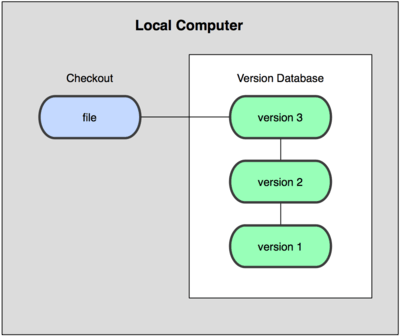
\includegraphics[scale=0.3]{VCS_local.png}\\
Not shared with anyone\\
e.g. on your own HDD
\column{.5\textwidth}
\centering
{\LARGE CENTRALIZED}\\[0.2in]
%{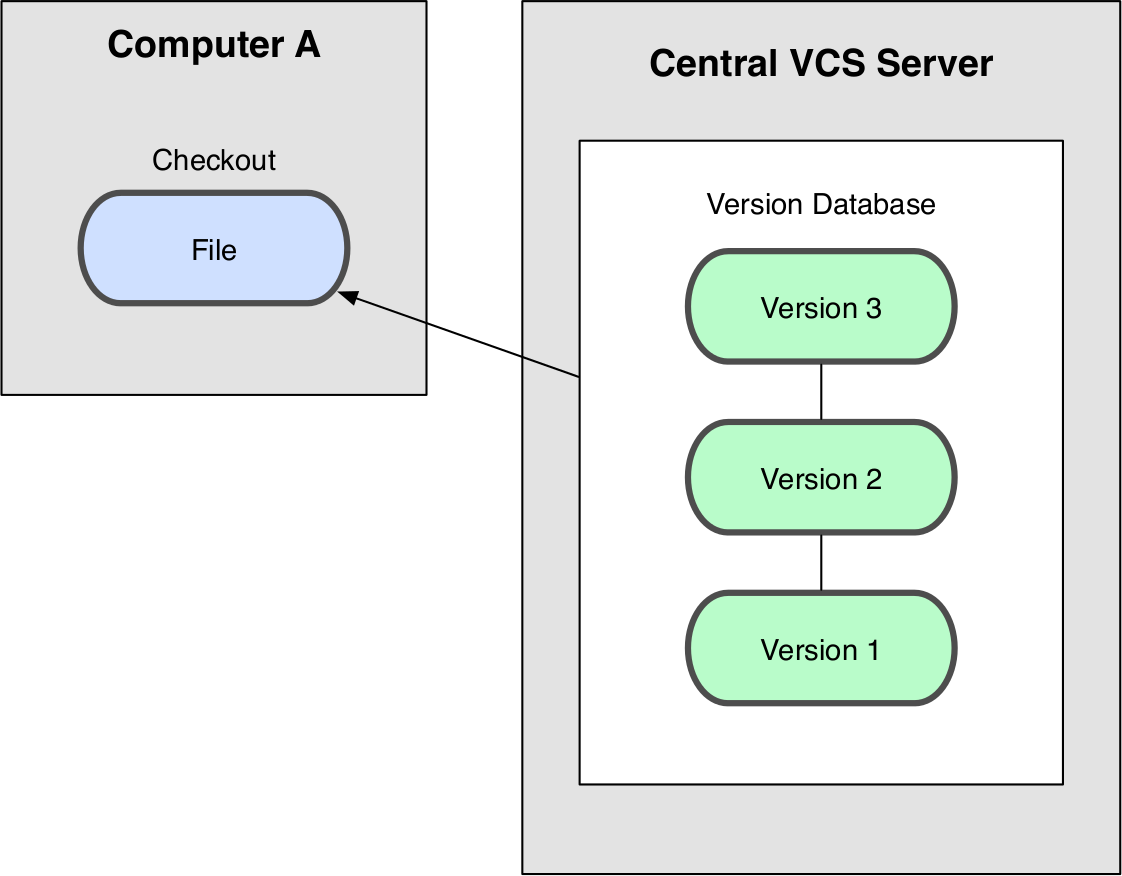
\includegraphics [scale=0.3]{VCS_centralized-1.png}}
{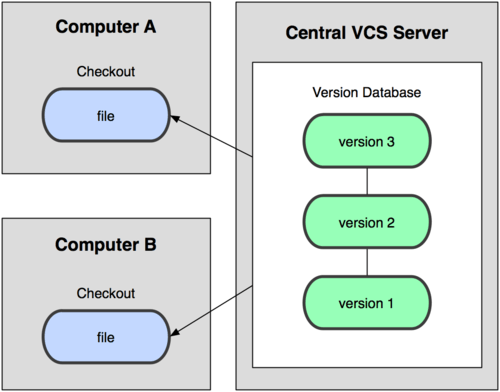
\includegraphics [scale=0.3]{VCS_centralized-2.png}}\\
Everybody sees the same version\\
on the server\\
\end{columns}
\end{frame}

\begin{frame}{Distributed VCS}{Git}

\begin{center}
\centering
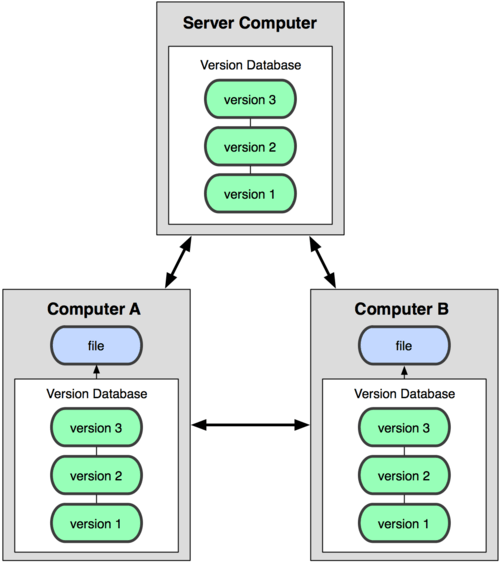
\includegraphics [scale=0.3]{VCS_distributed.png}\\[0.2in]
Both local AND global, but most operations are local\\
 Everybody has the full history of commits
\end{center}
\end{frame}


\begin{frame}{Some Typical VCS Workflows}
\begin{columns}
\column{.5\textwidth}
{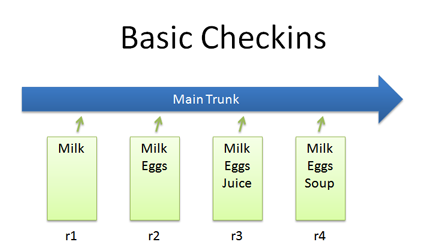
\includegraphics [scale=0.3]{basic_checkin.png}}
\pause
{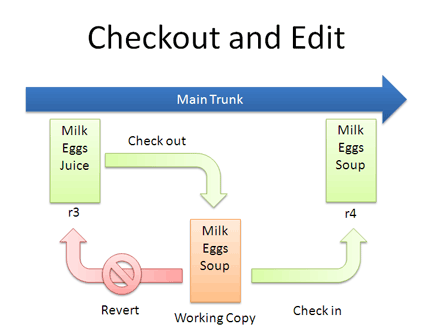
\includegraphics [scale=0.3]{checkout_edit.png}}
\pause
\column{.5\textwidth}
{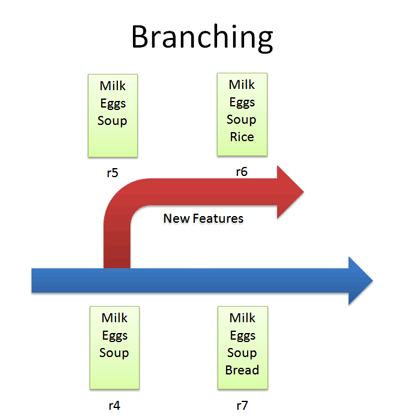
\includegraphics [scale=0.28]{first_branch.png}}
\pause
{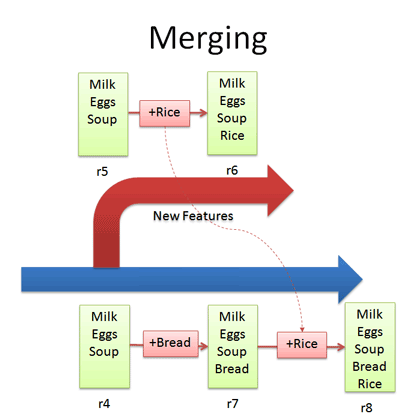
\includegraphics [scale=0.28]{merging.png}}
\end{columns}
\end{frame}

\subsection{Install}

\begin{frame}{Install git}
\begin{block}{Linux / UNIX}
     \begin{itemize}
       \setlength\itemsep{0.2in}
       \item {\bf OS X}\\ \$ brew install git %#\;\;\;\;\; #homebrew
       \item {\bf Ubuntu}\\ \$ aptitude install git
       \item {\bf Arch}\\ \$ pacman -S git
     \end{itemize}
\end{block}

\begin{block}{Windows}
    \begin{itemize}
      \item \url{https://git-for-windows.github.io/}
    \end{itemize}
\end{block}
\end{frame}

\subsection{Basic commands}

\begin{frame}{}
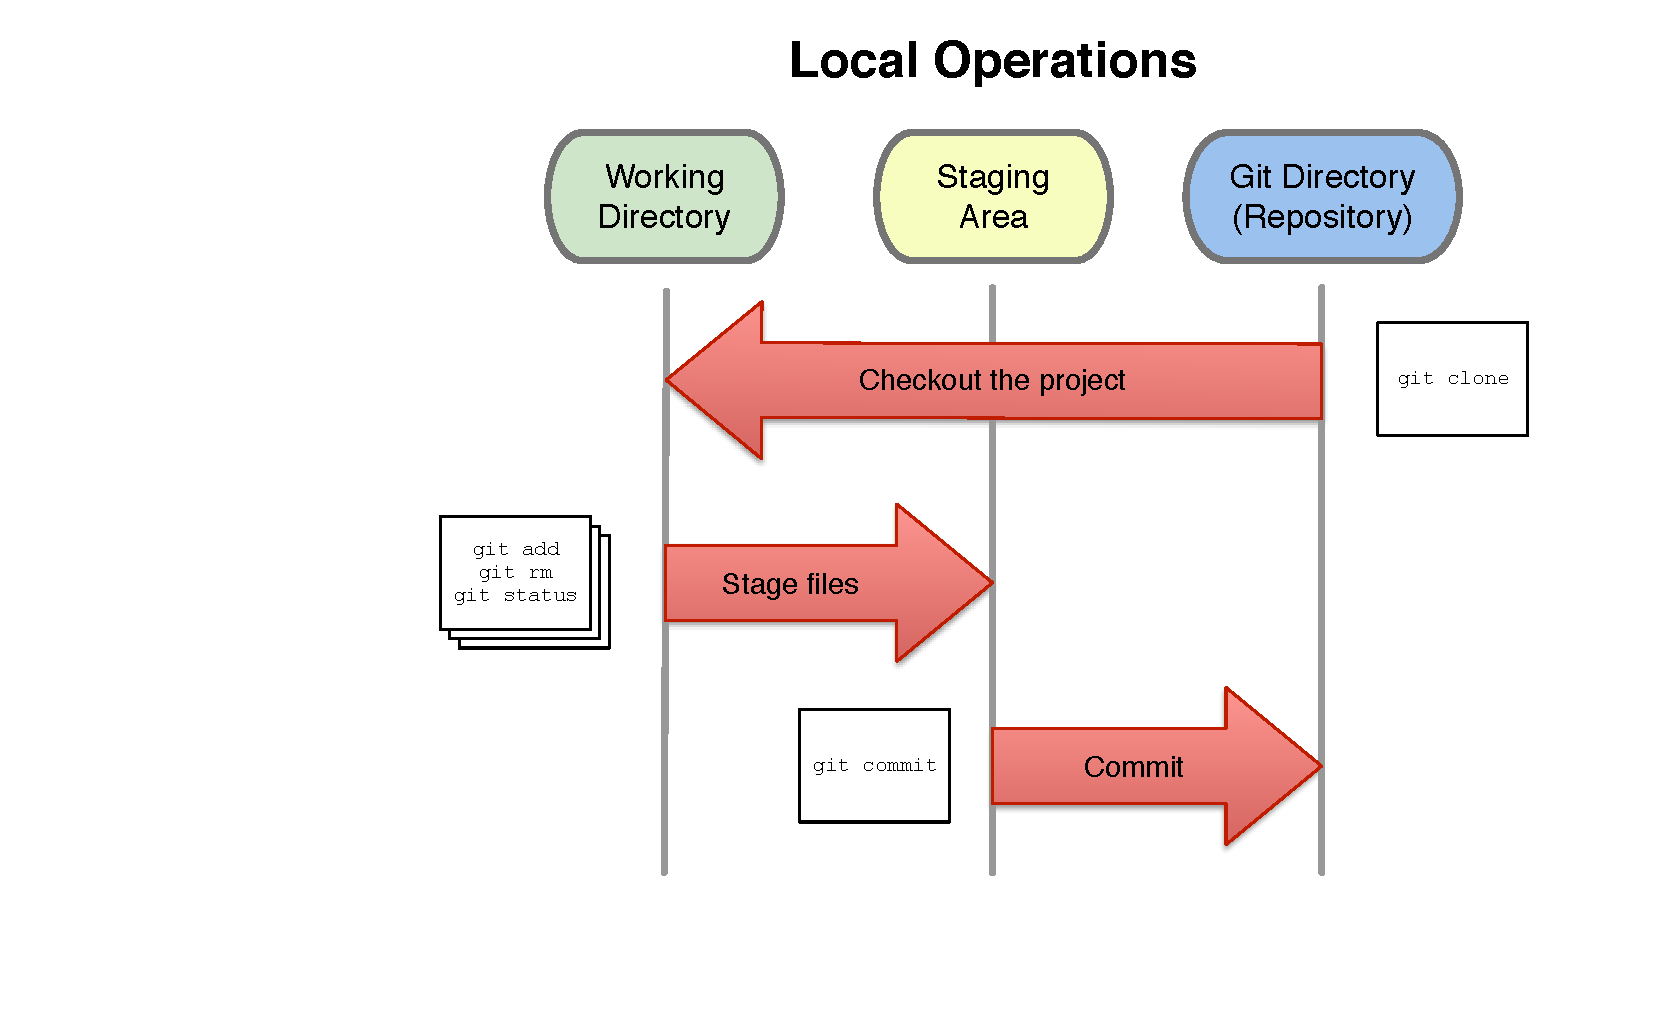
\includegraphics[width = 0.7\textwidth]{three_states.pdf}
\end{frame}

\begin{frame}{}
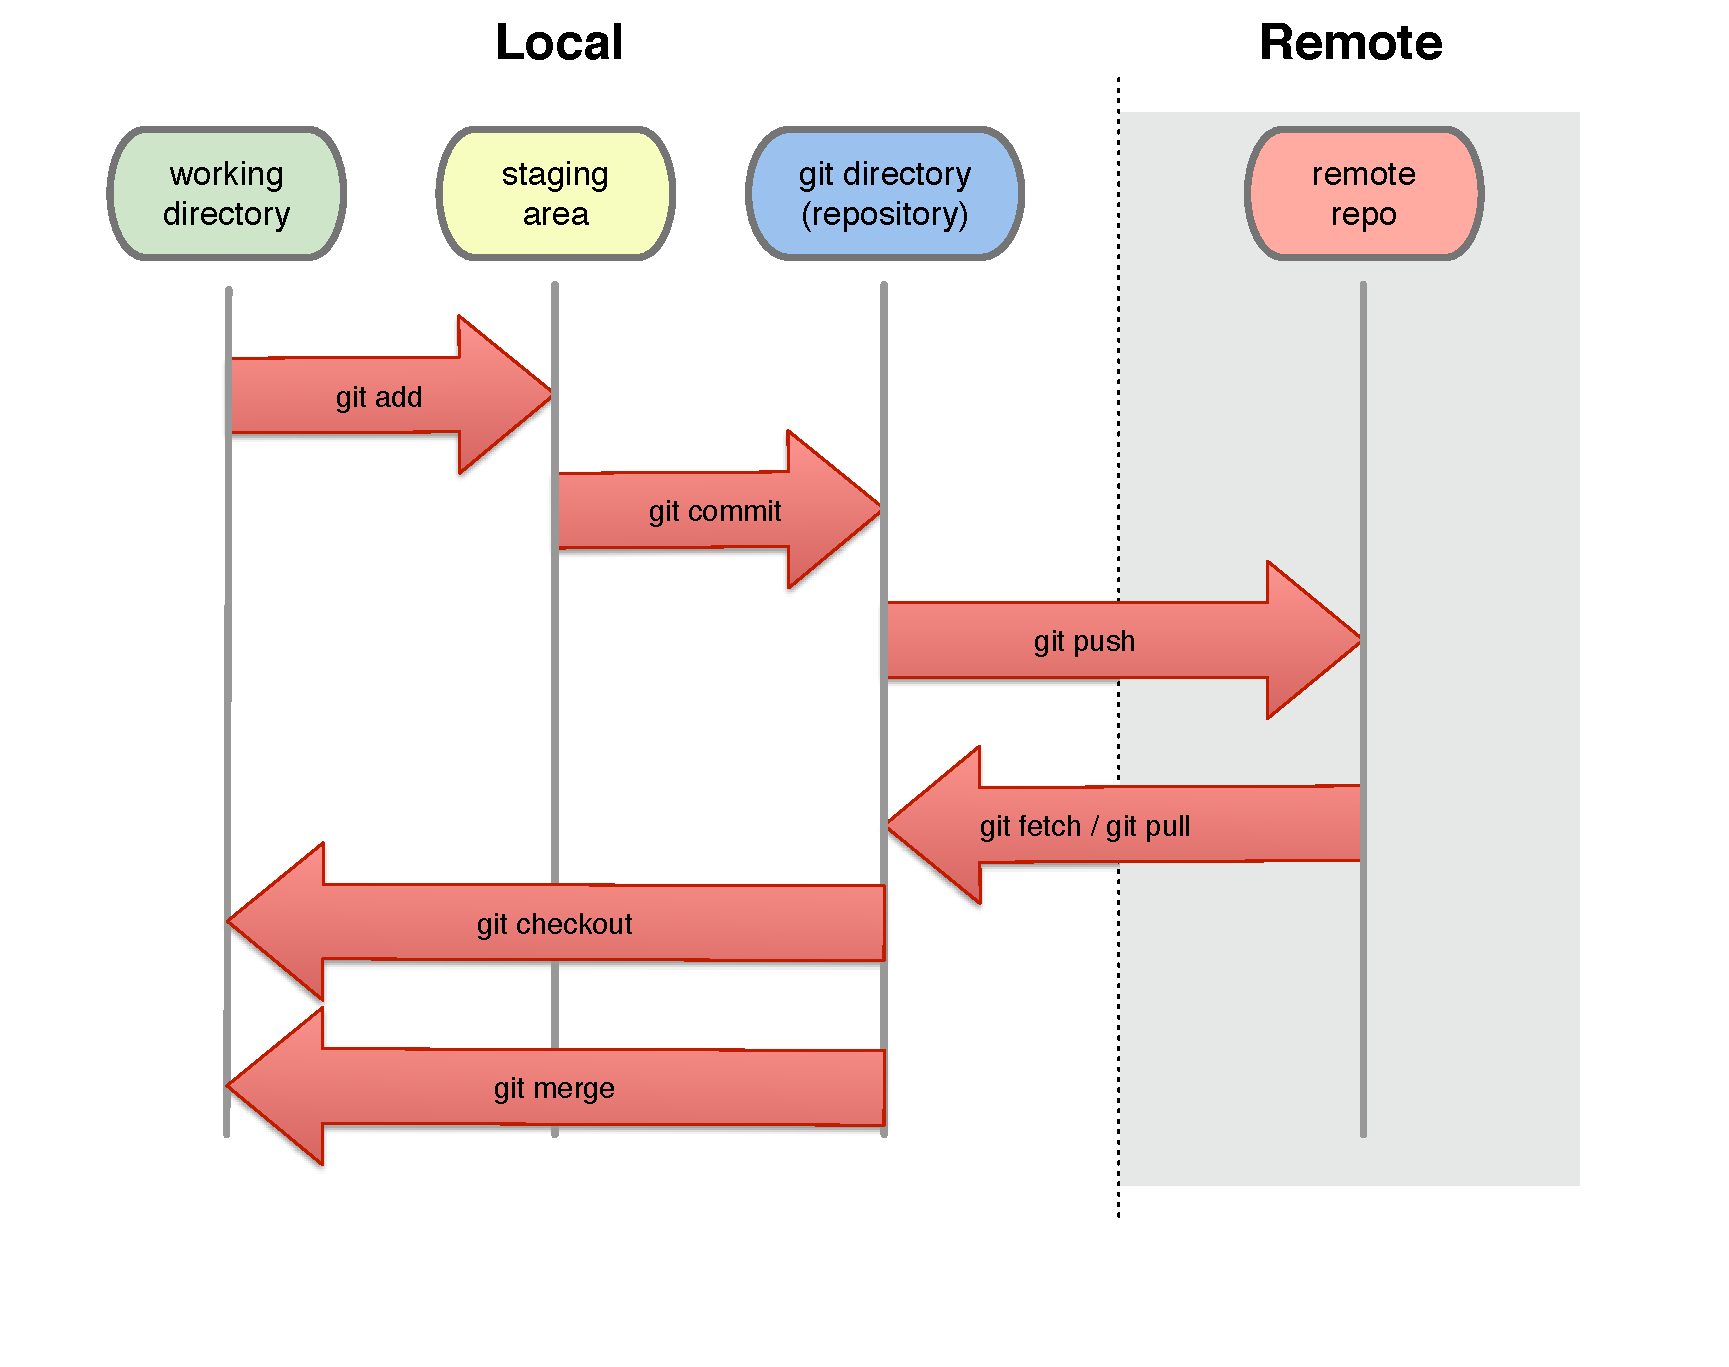
\includegraphics[width = 0.7\textwidth]{diagrams-lifecycle_remote.pdf}
\end{frame}

\section{Advanced topics}

\section{GitLab}

\section{Git resources}
\begin{frame}{Further reading}
\begin{itemize}
  \setlength\itemsep{0.4in}
\item "Pro Git" Book by ... \\$\rightarrow$  \url{http://git-scm.com/book}
\item Git reference  \\ $\rightarrow$  \url{http://git-scm.com/docs}
\item Git cheatsheet  \\ $\rightarrow$ \url{https://www.git-tower.com/blog/git-cheat-sheet}
\end{itemize}
\end{frame}

\begin{frame}{Learning by doing}
\begin{itemize}
  \setlength\itemsep{0.4in}
\item Tutorials  \\$\rightarrow$  \url{https://www.atlassian.com/git/tutorials}
\item Learn Git on codecademy - Strongly recommended!\\ $\rightarrow$ \url{https://www.codecademy.com/learn/learn-git}
\end{itemize}
\end{frame}



\end{document}

